\subsection{GPIOZero Python-Bibliothek / pinout Tool}

GPIOZero ist eine der vielen Python Bibliotheken, welche genutzt werden kann
um auf die GPIOs der Raspberry PI zuzugreifen. Sie wird unter der BSD Lizenz 
angeboten.

Das Paket beinhaltet auch das Kommandozeilentool 'pinout'. Dieses zeigt 
Hardwareinformationen und die Pin-Anordnung in der Kommandozeile an.

\begin{figure}[ht]
  \centering
  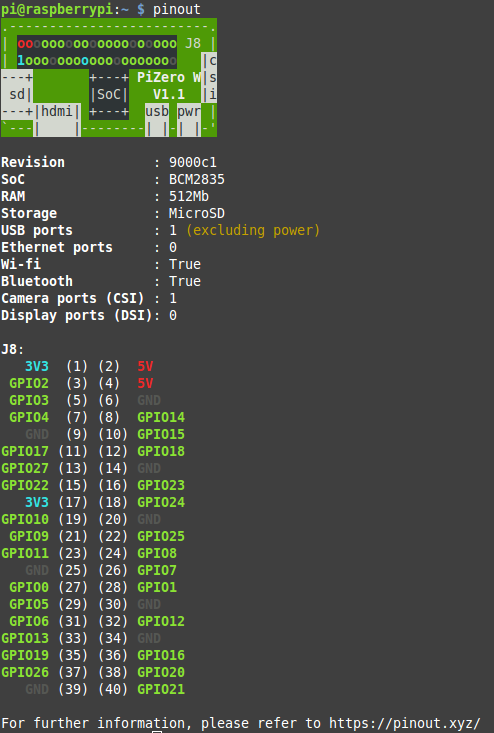
\includegraphics[scale=0.48]{images/Cmd_Pinout.png}
  \caption{Ergebnis des Kommandos 'pinout' in der Konsole}
  \label{CmdPinoutResult}
\end{figure}

Die Bezeichnung der Pins ist sehr wichtig, da es zwei unterschiedliche Arten 
gibt die Pins anzusprechen. Die GPIOZero Bibliothek verwendet ausschlie�lich
die Broadcom Nummerierung (BCM numbering) und dies kann auch nicht auf die
physikalische Nummerierung (BOARD numbering) umgestellt werden. D.h. will
man den physikalisch dritten Pin (direkt unter den 3.3V) schalten, muss man
wissen dass dieser die Bezeichnung GPIO2 besitzt und demzufolge die Pin-Nummer 2
besitzt.
